Cette partie contient de nombreux diagrammes permettant de décrire notre application.
\section{Diagramme de modèle du domaine}
\begin{figure}[h!]
\begin{center}
   \caption{Diagramme de modèle du domaine}
   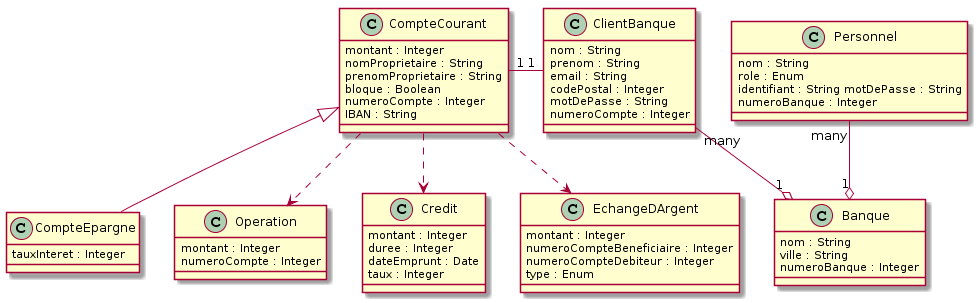
\includegraphics[scale=0.5]{modeleDuDomaine.png}
   \end{center}
\end{figure}
\newpage
\section{Diagramme d'activité de navigation}
\begin{figure}[h!]
\begin{center}
   \caption{Diagramme de navigation}
   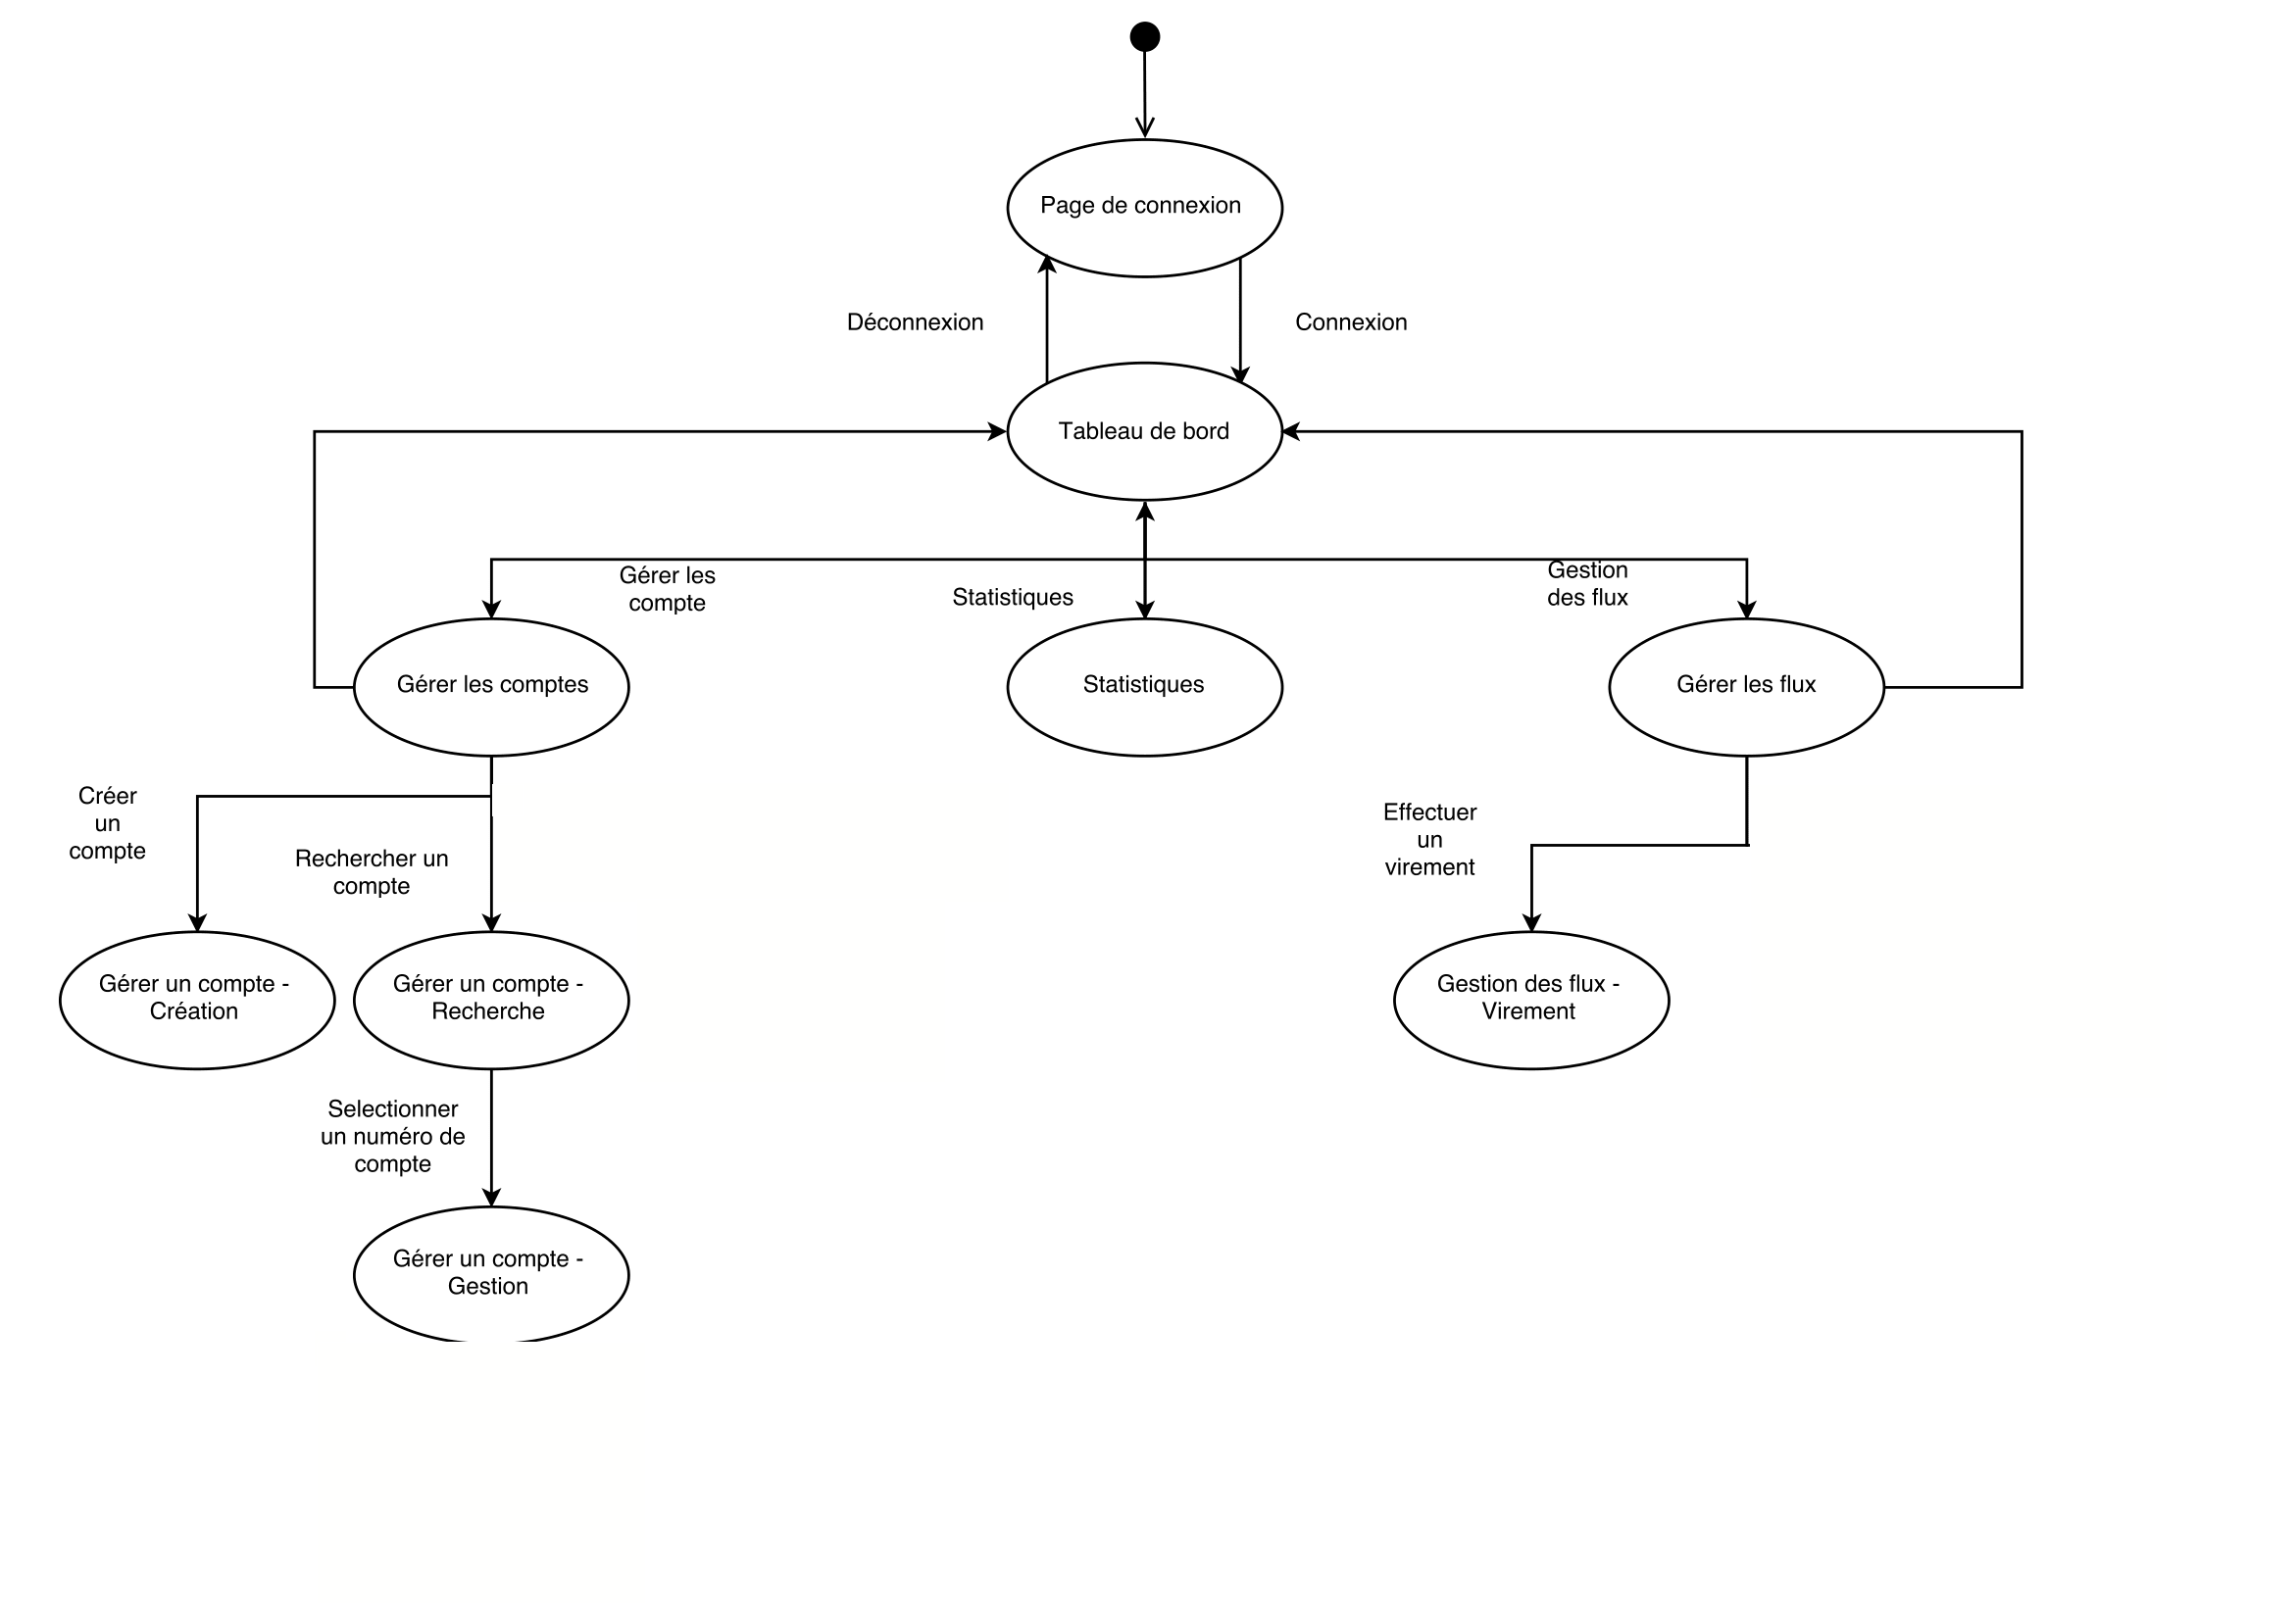
\includegraphics[scale=0.5]{navigation.pdf}
   \end{center}
\end{figure}
\newpage
\section{Diagrammes d'interaction}
\subsection{Cas d'utilisation : Se connecter}
\begin{figure}[h!]
\begin{center}
   \caption{Diagramme d'interaction : Se connecter}
   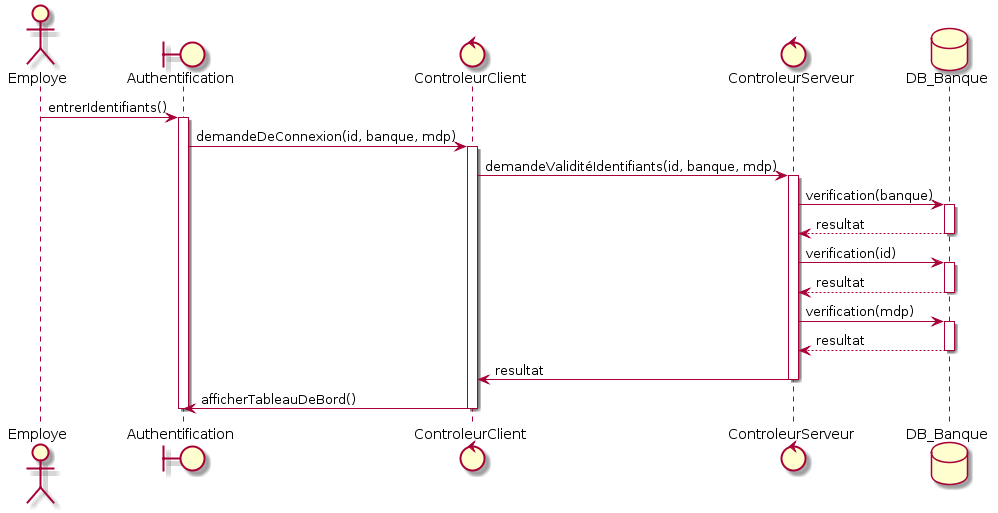
\includegraphics[scale=0.5]{seConnecterIR.png}
   \end{center}
\end{figure}
\subsection{Cas d'utilisation : Créer un compte}
\begin{figure}[h!]
\begin{center}
   \caption{Diagramme d'interaction : Créer un compte}
   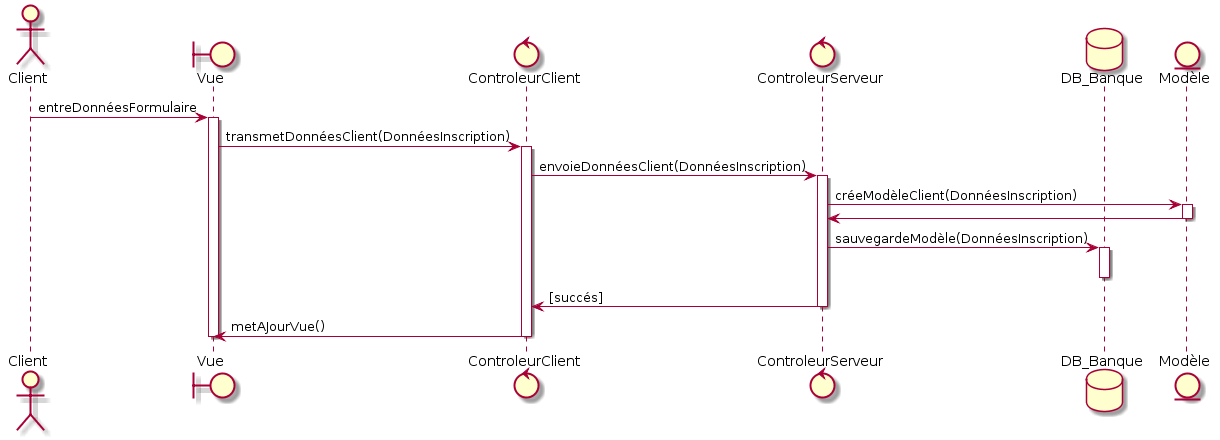
\includegraphics[scale=0.4]{SInscrire.png}
   \end{center}
\end{figure}
\newpage
\section{Diagramme de classes de conception préliminaire}
\begin{figure}[h!]
\begin{center}
   \caption{Diagramme de classes}
   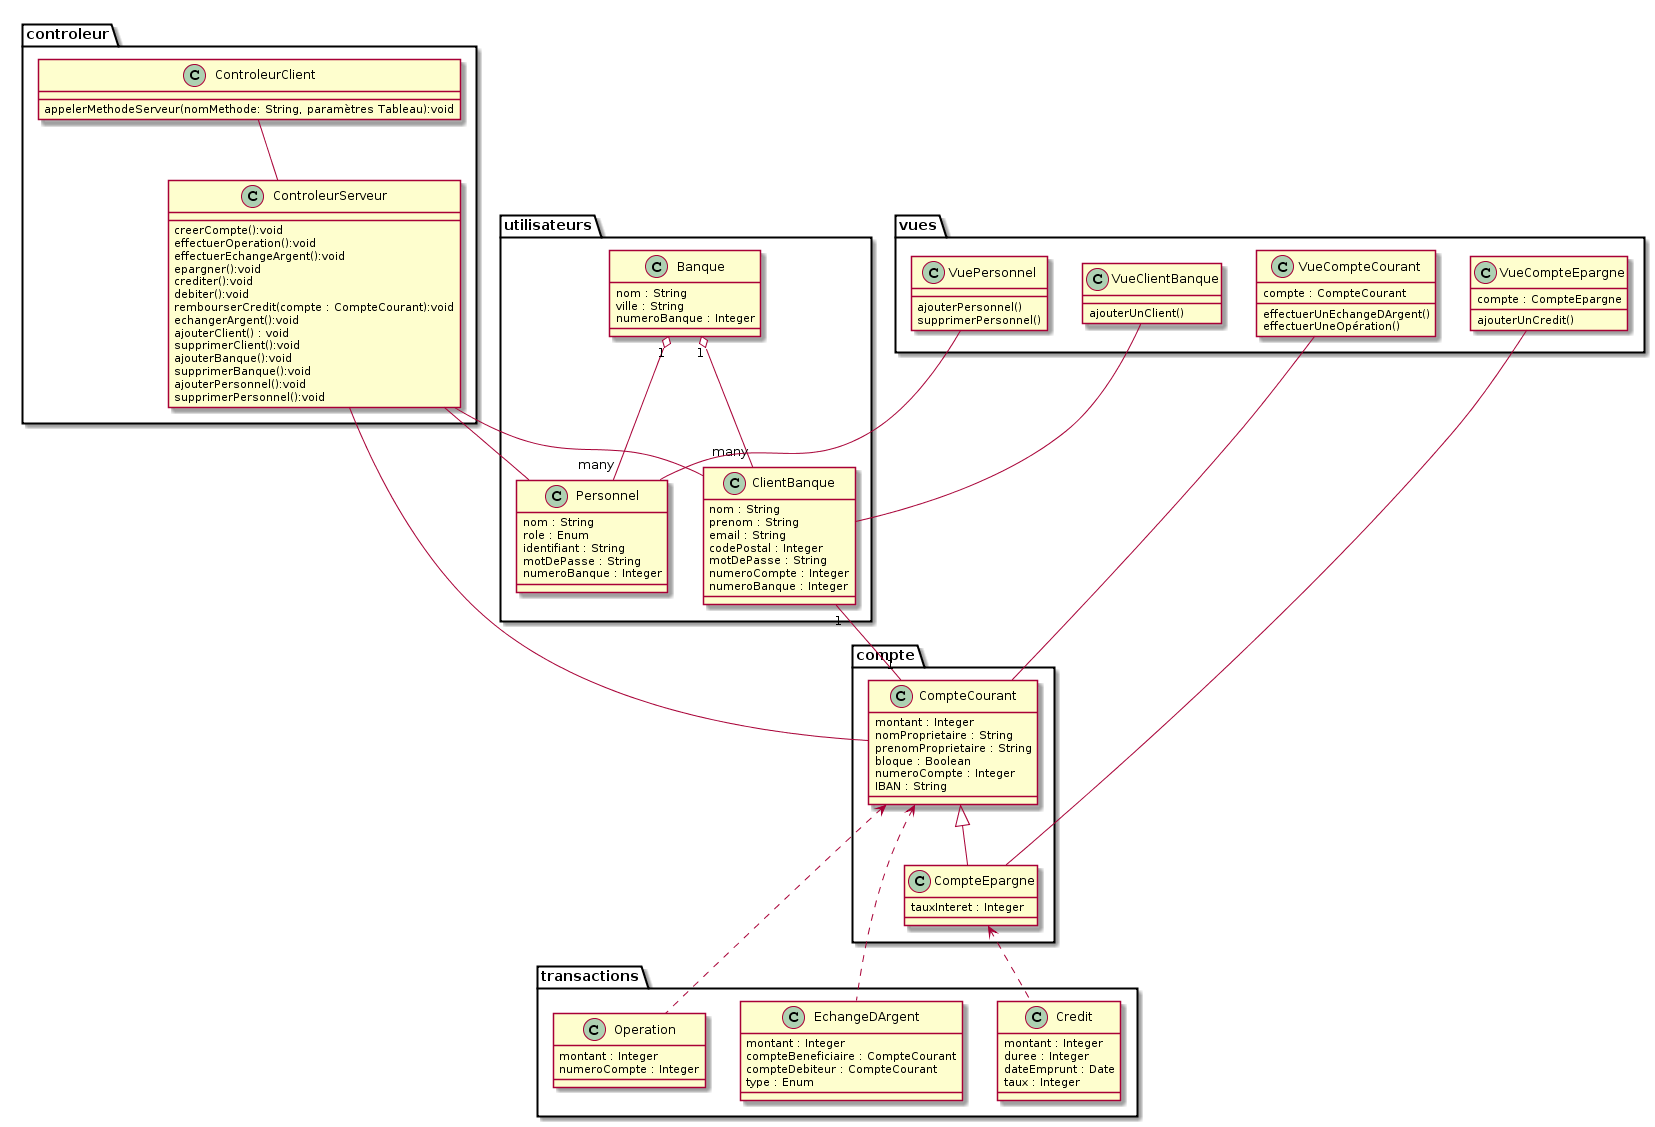
\includegraphics[scale=0.3, angle=90]{diagrammeClasses.png}
   \end{center}
\end{figure}